% ------------------------------------------------------------------------------
\documentclass[final, 12pt]{beamer}


% ========================================================================================
% Theme: inner, outer, font and colors
% ----------------------------------------------------------------------------------------
\usepackage[institute=Nat,
			%WordMark=None
			ExtraLogo = template-art/DepartMath.pdf,
			size=a0,
			signature=tim.roith@fau.de
		   ]{styles/beamerposterthemefau}
% ----------------------------------------------------------------------------------------
% Input and output encoding
\usepackage[T1]{fontenc}
\usepackage[utf8]{inputenc}
% ----------------------------------------------------------------------------------------
% Language settings
\usepackage[english]{babel}


% ========================================================================================
% Fonts
% - Helvet is loaded by styles/beamerfonts
% - We use serif for math environements
% - isomath is used for upGreek letters
% ----------------------------------------------------------------------------------------
\usepackage{isomath}
\usefonttheme[onlymath]{serif}
\usepackage{exscale}
\usepackage{anyfontsize}
\setbeamercolor{alerted text}{fg=BaseColor}
% ----------------------------------------------------------------------------------------
% custom commands for symbols
\usepackage{styles/symbols}


% ========================================================================================
% Setup for Titlepage
% ----------------------------------------------------------------------------------------
\title[]{A Bregman Learning Framework for
Sparse Neural Networks}
\subtitle{Training neural networks via mirror descent}
\author[T. Roith]{Leon Bungert, Tim Roith, Daniel Tenbrinck, Martin Burger}
\institute[FAU]{Friedrich-Alexander Universität Erlangen-Nürnberg, Department Mathematik}
\date{\today}


% ========================================================================================
% Bibliography
% ----------------------------------------------------------------------------------------
\usepackage{csquotes}
\usepackage[style=alphabetic, %alternatively: numeric, numeric-comp, and other from biblatex
			defernumbers=true,
			useprefix=true,%
			giveninits=true,%
			hyperref=true,%
			autocite=inline,%
			maxcitenames=5,%
			maxbibnames=20,%
			uniquename=init,%
			sortcites=true,% sort citations when multiple entries are passed to one cite command
			doi=true,%
			isbn=false,%
			url=false,%
			eprint=false,%
			backend=biber%
		   ]{biblatex}
\addbibresource{bibliography.bib}
\setbeamertemplate{bibliography item}[text]


% ========================================================================================
% Hyperref and setup
% ----------------------------------------------------------------------------------------
\usepackage{hyperref}
\hypersetup{
	colorlinks = true,
	final=true, 
	plainpages=false,
	pdfstartview=FitV,
	pdftoolbar=true,
	pdfmenubar=true,
	pdfencoding=auto,
	psdextra,
	bookmarksopen=true,
	bookmarksnumbered=true,
	breaklinks=true,
	linktocpage=true,
	urlcolor=BaseColor,
	citecolor=BaseColor,
	linkcolor=BaseColor
}


% ========================================================================================
% Additional packages
% ----------------------------------------------------------------------------------------
\usepackage{subcaption}


% ========================================================================================
% Various custom commands
% ----------------------------------------------------------------------------------------
\pdfsuppresswarningpagegroup=1 %solves the PDF inclusion problem
% Change color for cite locally
\newcommand{\colorcite}[3]{{\hypersetup{citecolor=#1}{\cite[#2]{#3}}}}
\setlength{\abovedisplayskip}{0pt}
% ----------------------------------------------------------------------------------------
% ========================================================================================
% The main document
% ----------------------------------------------------------------------------------------
\begin{document}
\begin{frame}{-}{}
%
\newlength\colwidth
\newlength\topstripheight
\setlength{\colwidth}{.49\textwidth}
\setlength{\topstripheight}{.4\textheight}
% -----------------------------------------------------------------------
\hbox to \textwidth{%
\tbox{%
% ---------------------------------------------------
% Left side: Intro
% ---------------------------------------------------
\begin{minipage}[t]{\colwidth}%
\vskip 0pt%
% ---------------------------------------------------
\begin{figure}[tb]
\def\PicWidth{0.24\textwidth}%
\centering%
\begin{subfigure}[b]{\PicWidth}
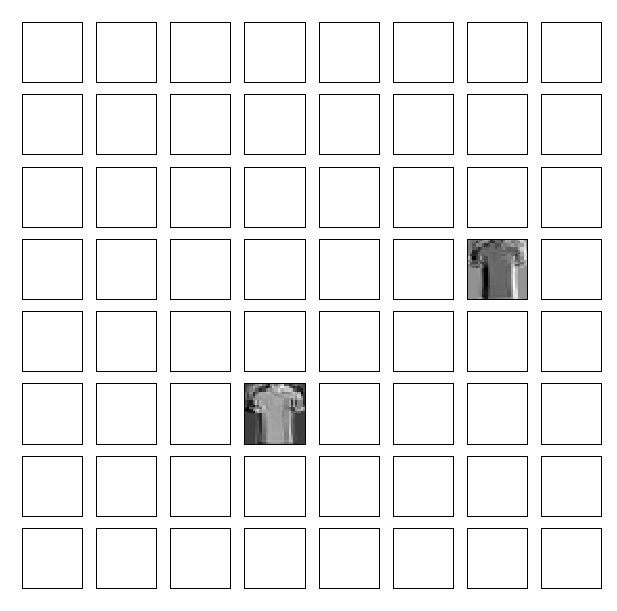
\includegraphics[width=\textwidth,trim=0.35cm 0.35cm 0.2cm 0.35cm,clip]{atelier/FMNIST/FM_e0.pdf}%
\caption{Iteration 0}
\end{subfigure}
\hfill%
%
\begin{subfigure}[b]{\PicWidth}
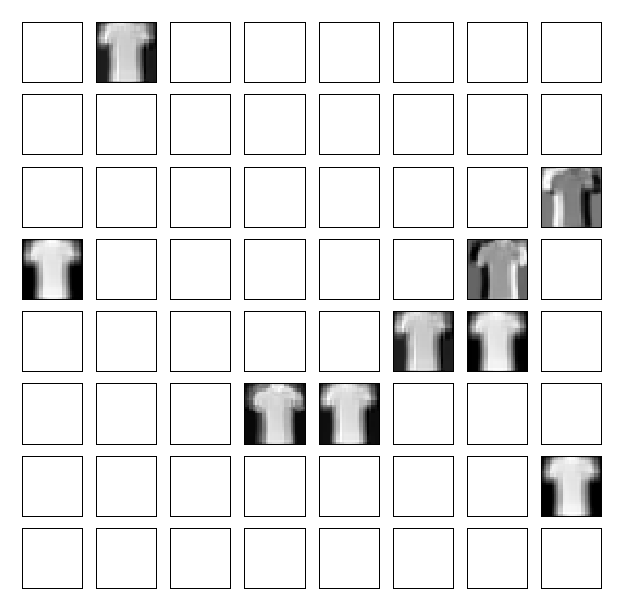
\includegraphics[width=\textwidth,trim=0.35cm 0.35cm 0.2cm 0.35cm,clip]{atelier/FMNIST/FM_e5.pdf}%
\caption{Iteration 5}
\end{subfigure}
\hfill%
%
\begin{subfigure}[b]{\PicWidth}
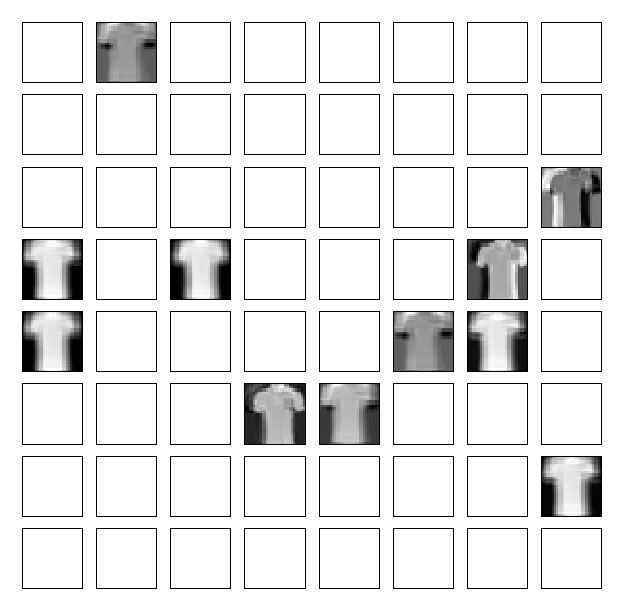
\includegraphics[width=\textwidth,trim=0.35cm 0.35cm 0.2cm 0.35cm,clip]{atelier/FMNIST/FM_e20.pdf}%
\caption{Iteration 20}
\end{subfigure}
\hfill%
%
\begin{subfigure}[b]{\PicWidth}
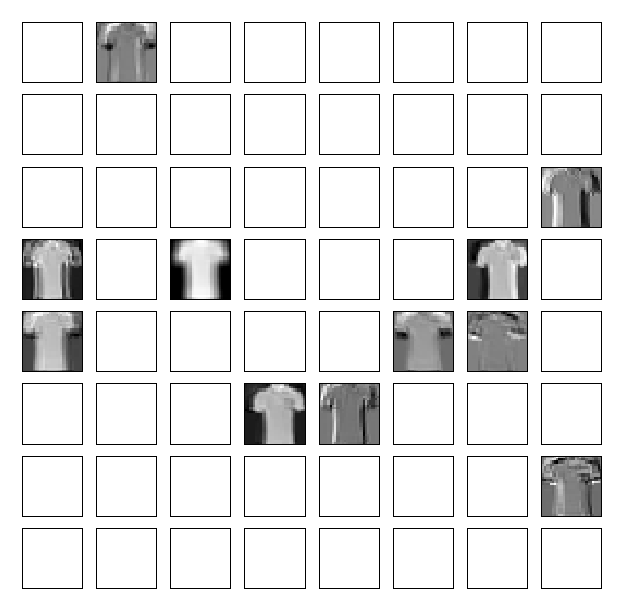
\includegraphics[width=\textwidth,trim=0.35cm 0.35cm 0.2cm 0.35cm,clip]{atelier/FMNIST/FM_e100.pdf}%
\caption{Iteration 100}
\end{subfigure}
\caption{Inverse scale space character of \LinBreg{} visualized through feature maps of a convolutional neural network. 
Descriptive kernels are gradually added in the training process.}
\label{fig:kernels}
\vspace{-10pt}
\end{figure}
% ---------------------------------------------------
%
%
%
%
\cblock{BaseColor}{}{Bregman Training in a Nutshell}{%
\small
For input and output spaces $\Inp, \Oup$ we denote by $\net_\param:\Inp\to\Oup$ a neural network parameterized by $\param$ from some parameter space $\Param$. For a feed-forward have that $\net_\param = \Phi^L\circ\ldots\circ\Phi^1$ where the $l$-th layer is given by
%
\begin{align*}
\Phi^L: x\mapsto \sigma\left(W^l x + b^l\right).
\end{align*}
Here, $W^l, b^l$ denote the weights and biases of the $l$-th layer and $\sigma$ is an activation function.
}
\vspace{.5em}

%
\begin{minipage}[t]{.48\textwidth}%
\small%
We are interested in finding parameters that minimize some \textcolor{BaseDarkColor}{\textbf{loss}} $\empLoss:\Param\to\R$. This is done via a gradient-based method, where in each step we replace the loss 



% training data $\trSet\subset \Inp\times\Oup$ want typically replaces 
\end{minipage}%
%
\hfill%
%
\begin{minipage}[t]{.48\textwidth}%
\small%
Additionally, we want the parameters to be \textcolor{BaseDarkColor}{\textbf{sparse}} which is enforced, via an regularization functional $\func:\Param\to\R$.
\end{minipage}%


%
\begin{minipage}[t]{\textwidth}%
\cblock{BaseColor}{}{The Algorithm}{%
\small%
Embedding linearized Bregman iterations in a stochastic framework, we denote by $g:\Param\times\Omega \to \Param$ an unbiased estimator of $\nabla\empLoss$, i.e., $\Exp{g(\param;\omega)} = \nabla\empLoss(\param)$ for some probability space $(\Omega, \P)$. In each step we sample $\omega^k$ from $\P$, set $g^k = g(\theta^k; \omega^k)$ and perform the following update
%
\begin{block}{}%
\begin{align*}%
v^{k+1} &:= v^{k} - \tau^{k} g^{k},\qquad&\text{Gradient Step}\\
\param^{k+1} &:= \prox{\delta J}(\delta v^{k+1}).
\qquad&\text{Proximal Step}
\end{align*}%
\end{block}%
}%
\end{minipage}%
\end{minipage}%
}%
%
%
%
%
% ---------------------------------------------------
% Line Divider
% ---------------------------------------------------
\hfill%
%
\tbox{%
\begin{minipage}[t]{.005\textwidth}%
\vskip 0pt%
\begin{center}
\textcolor{BaseDarkColor}{%
\rule{.2mm}{\topstripheight}%
}
\end{center}
\end{minipage}%
}%
%
\hfill%
%
%
%
%
%
% ---------------------------------------------------
% Analytical Results
% ---------------------------------------------------
\tbox{%
\begin{minipage}[t]{\colwidth}%
\vskip 0pt%
\cblock{BaseColor}{}{Assumptions}{}%
%Section for assumptions
\begin{minipage}{\textwidth}%
\small%
\begin{minipage}[t]{.48\textwidth}%
\cblock{BaseColorA}{}{Assumption 1: The Loss function}{%
We assume that $\empLoss\geq 0$, $\empLoss$ is continuously differentiable and that for all $\param,\tilde\param\in\Param$ we have
\begin{align*}
\norm{\nabla\empLoss(\tilde\param)-\nabla\empLoss(\param)}\leq L \norm{\tilde\param-\param}.
\end{align*}%
}%
\end{minipage}%
%
\hfill
%
\begin{minipage}[t]{.48\textwidth}%
\cblock{BaseColorA}{}{Assumption 2: Bounded Variance}{%
There exists a constant $\sigma>0$ such that for any $\param\in\Param$ it holds
\begin{align*}
\E\left[\norm{g(\param;\omega)-\nabla\empLoss(\param)}^2\right] \leq \sigma^2.
\end{align*}%
}%
\end{minipage}%
\end{minipage}%
%
\vspace{.5em}

%
\begin{minipage}{\textwidth}%
\small%
\begin{minipage}[t]{.48\textwidth}%
\cblock{BaseColorA}{}{Assumption 3: Regularizer}{%
We assume that $\func:\Param\to(-\infty,\infty]$ is a convex, proper, and lower semicontinuous functional on the Hilbert space $\Param$.%
}%
\end{minipage}%
%
\hfill%
%
\begin{minipage}[t]{.48\textwidth}%
\cblock{BaseColorA}{}{Assumption 4: Strong Convexity}{%
We have that for all $\param,\tilde\param\in\Param$
\begin{align*}
\empLoss(\tilde\param) &\geq \empLoss(\param) + \langle\nabla\empLoss(\param),\tilde\param - \param\rangle\\
&+ \frac{\mu}{2}\norm{\tilde\param-\param}^2.
\end{align*}%
}%
\end{minipage}%
\end{minipage}%
\vspace{1em}

%
%
%
%
\cblock{BaseColor}{}{Loss Decay}{%
% section for loss decay
\small
Assume that Assumptions 1--3 hold true, let $\delta>0$, and let the step sizes satisfy $\tau^{(k)} \leq \frac{2}{\delta L}$.
Then there exist constants $c,C>0$ such that for every $k\in\N$ the iterates of (??) satisfy
\begin{block}{}
\begin{align*}
\textcolor{BaseColor}{\E\left[\empLoss(\param^{(k+1)})\right]} &+
%
\frac{1}{\tau^{(k)}}\E\left[ D^\mathrm{sym}_\func(\param^{(k+1)},\param^{(k)})\right]\\
%
&+
\frac{C}{2\delta\tau^{(k)}}\E\left[\norm{\param^{(k+1)}-\param^{(k)}}^2\right] %\\
%
\leq
\textcolor{BaseColor}{\E\left[\empLoss(\param^{(k)})\right]} + \tau^{(k)}\delta\frac{\sigma^2}{2c}.
\end{align*}
\end{block}
}%
%
%
%
\cblock{BaseColor}{}{Convergence in Norm}{%
\small%
Assume that Assumptions 1--4 hold true and that $J(\param^*)<\infty$, where  $\param^*$ is the unique minimizer of $\mathcal{L}$. For every $k\in\N$ and  $d_k:=\E\left[D_{\func_\delta}^{v^{(k)}}(\param^*,\param^{(k)})\right]$ we have
%
\begin{block}{}
\begin{align*}
d_{k+1} - d_k
+ \frac{\mu}{4}\tau^{(k)}\E\left[\norm{\param^*-\param^{(k+1)}}^2\right]
%
\leq  \frac{\sigma}{2}\left((\tau^{(k)})^2 +\Exp{\norm{\param^{(k)} - \param^{(k+1)}}^2}\right).
\end{align*}
\end{block}
%
Furthermore, there exists a subsequence $\param^{(k_j)}$ such that
\begin{align*}
\lim_{j\to\infty}\E\left[\norm{\param^*-\param^{(k_j)}}^2\right] = 0.
\end{align*}
}%
\end{minipage}%
}%
}

\fbox{%
\begin{minipage}{\textwidth}
Seperator
\end{minipage}%
}%



%
\begin{minipage}{\textwidth}
\vskip0pt%
\textcolor{BaseColor}{%
\rule{\textwidth}{.2mm}%
}%
\end{minipage}%

%
%
%
%
\begin{minipage}[t]{\textwidth}%
\begin{center}
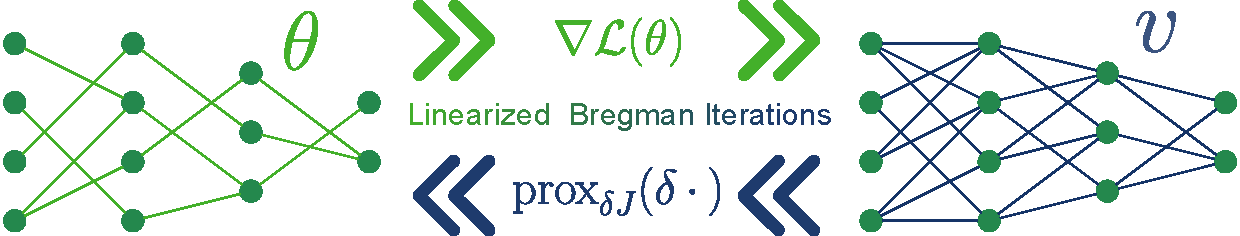
\includegraphics[height=8em]{atelier/BregmanPosterCartoon.pdf}
\end{center}
\end{minipage}%

%
%
%
%
%

%
\newlength\bottomstripheight%
\setlength{\bottomstripheight}{.25\textheight}%
%
\begin{minipage}[t]{\textwidth}%
\vskip0pt%
\textcolor{BaseColor}{%
\rule{\textwidth}{.2mm}%
}\hfill%
%
%
\begin{minipage}[b][\bottomstripheight][b]{.48\textwidth}%
%
\cblock{BaseColor}{}{Training results}{}%
\small%
\begin{figure}
\centering
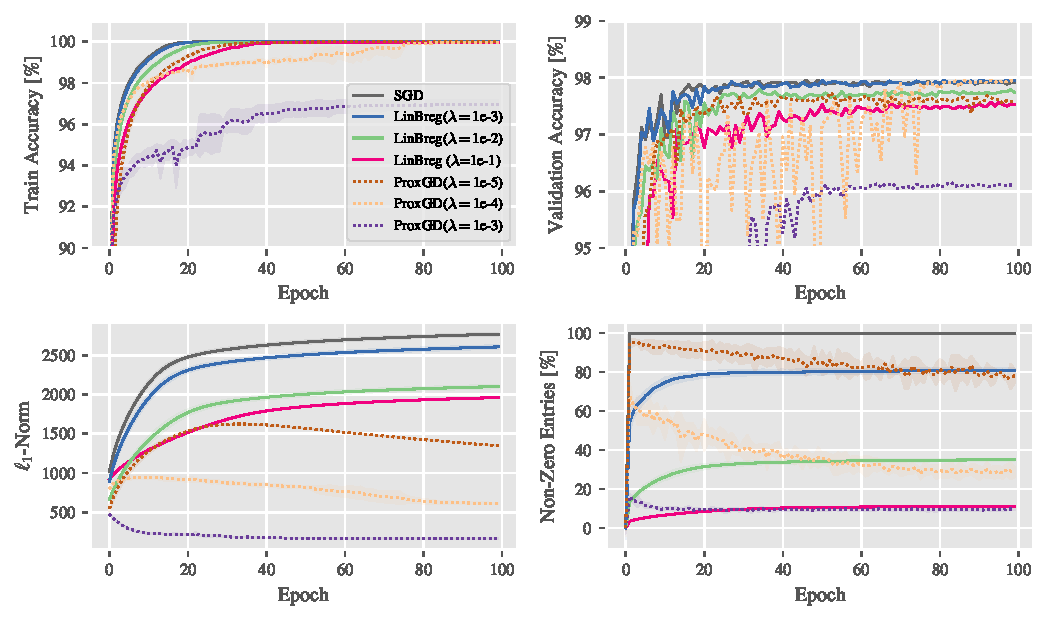
\includegraphics[width=.7\textwidth]{atelier/SGDvsBreg.pdf}
\caption{Comparison of vanilla SGD (black solid line), \LinBreg{} (colored solid lines), and ProxGD (colored dotted lines) for different regularization parameters on MNIST.
The curves show the averaged accuracies on train and validation sets, $\ell_1$-norms, and non-zero entries over three runs. The shaded area visualizes the standard deviation.}
\end{figure}%
\vfill%
\vphantom{.}
\end{minipage}%
%
\hfill%
%
\tbox{%
\noindent\begin{minipage}[b][\bottomstripheight][b]{.005\textwidth}%
%
\begin{center}
\textcolor{BaseColor}{%
\rule{.2mm}{\bottomstripheight}%
}
\end{center}
\end{minipage}%
}%
%
\hfill%
%
%
%
%
%
%
%
\noindent\begin{minipage}[b][\bottomstripheight][b]{.48\textwidth}%
%
\cblock{BaseColor}{}{NAS with Bregman}{}%
\small%


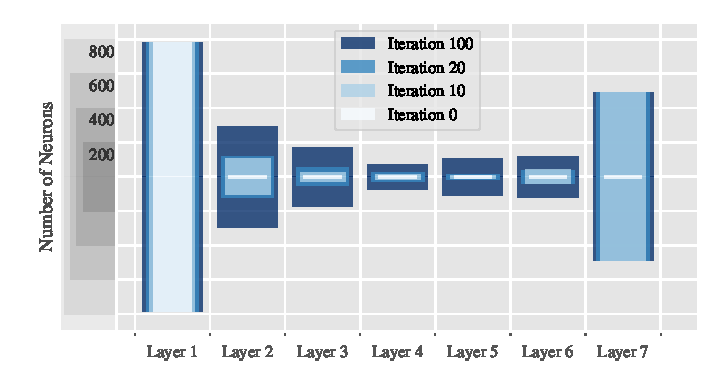
\includegraphics[width=\textwidth]{atelier/Encoder_3.pdf}
\vfill%
\vphantom{.}
\end{minipage}%
\end{minipage}%
%


%
\end{frame}
\end{document}